% Experiment

В этом разделе представлены результаты замеров производительности разработанного решения.

\subsection{Условия эксперимента}

При проведении экспериментального исследования использовался компьютер со следующими характеристиками: процессор Intel Core i7-10750H $6\times2.60$ GHz, 16 Gb DDR4 RAM. 

В качестве исходных данных были взяты RDF графы из репозитория CFPQ\_Data, которые собраны на реальных данных. Из репозитория выбирались графы, которые содержат хотя бы 10 уникальных меток на ребрах. Это условие требовалось для генерации более сложных запросов к этим графам. Такому условию удовлетворяют в большинстве своем графы, собранные на  биологических данных.

Характеристики выбранных графов представлены в таблице~\ref{table:dataset}.

\begin{table}[!ht]\caption{Датасет}\label{table:dataset}
    \centering
    \begin{tabular}{|l|l|l|}
    \hline
\rowcolor{lightgray}        Graph & \# Vertices & \# Edges \\ \hline
        core & 1 323 & 2 752 \\ \hline
        enzyme & 48 815 & 86 543 \\ \hline
        eclass & 239 111 & 360 248 \\ \hline
        go & 582 929 & 1 437 437 \\ \hline
    \end{tabular}
\end{table}

Регулярные запросы к графам были сгенерированы на основе самых популярных шаблонов запросов, собранных в  работе~\cite{experiment_shemetova2021}. Для каждого графа отбиралось 10 самых популярных меток, после чего по ним на основе шаблонов генерировалось случайным образом 5 запросов. В общей сложности по 23 шаблонам было сгенерировано 115 запросов к каждому графу.

В ходе проведения эксперимента каждый запрос исполнялся 5 раз, после чего вычислялось среднее значение исполненных запросов.

Всего было произведено 6 экспериментов: 1 эксперимент оценивающий эффективность алгоритма для одной исходной вершины (single source) и 5 экспериментов для нескольких стартовых вершин (multiple source).
Для single source эксперимента 1000 раз, не повторяясь, выбиралась одна стартовая вершина. Для multiple source эксперимента выбиралось случайное множество, состоящее из 10, 50, 100, 500 или 1000 стартовых вершин.

\subsection{Результаты}
Результаты эксперимента представлены на рисунке~\ref{fig:experiment}, где штрихами обозначены медианы для каждого из запросов.

\begin{figure}[ht]
  \noindent\makebox[\textwidth]{%
  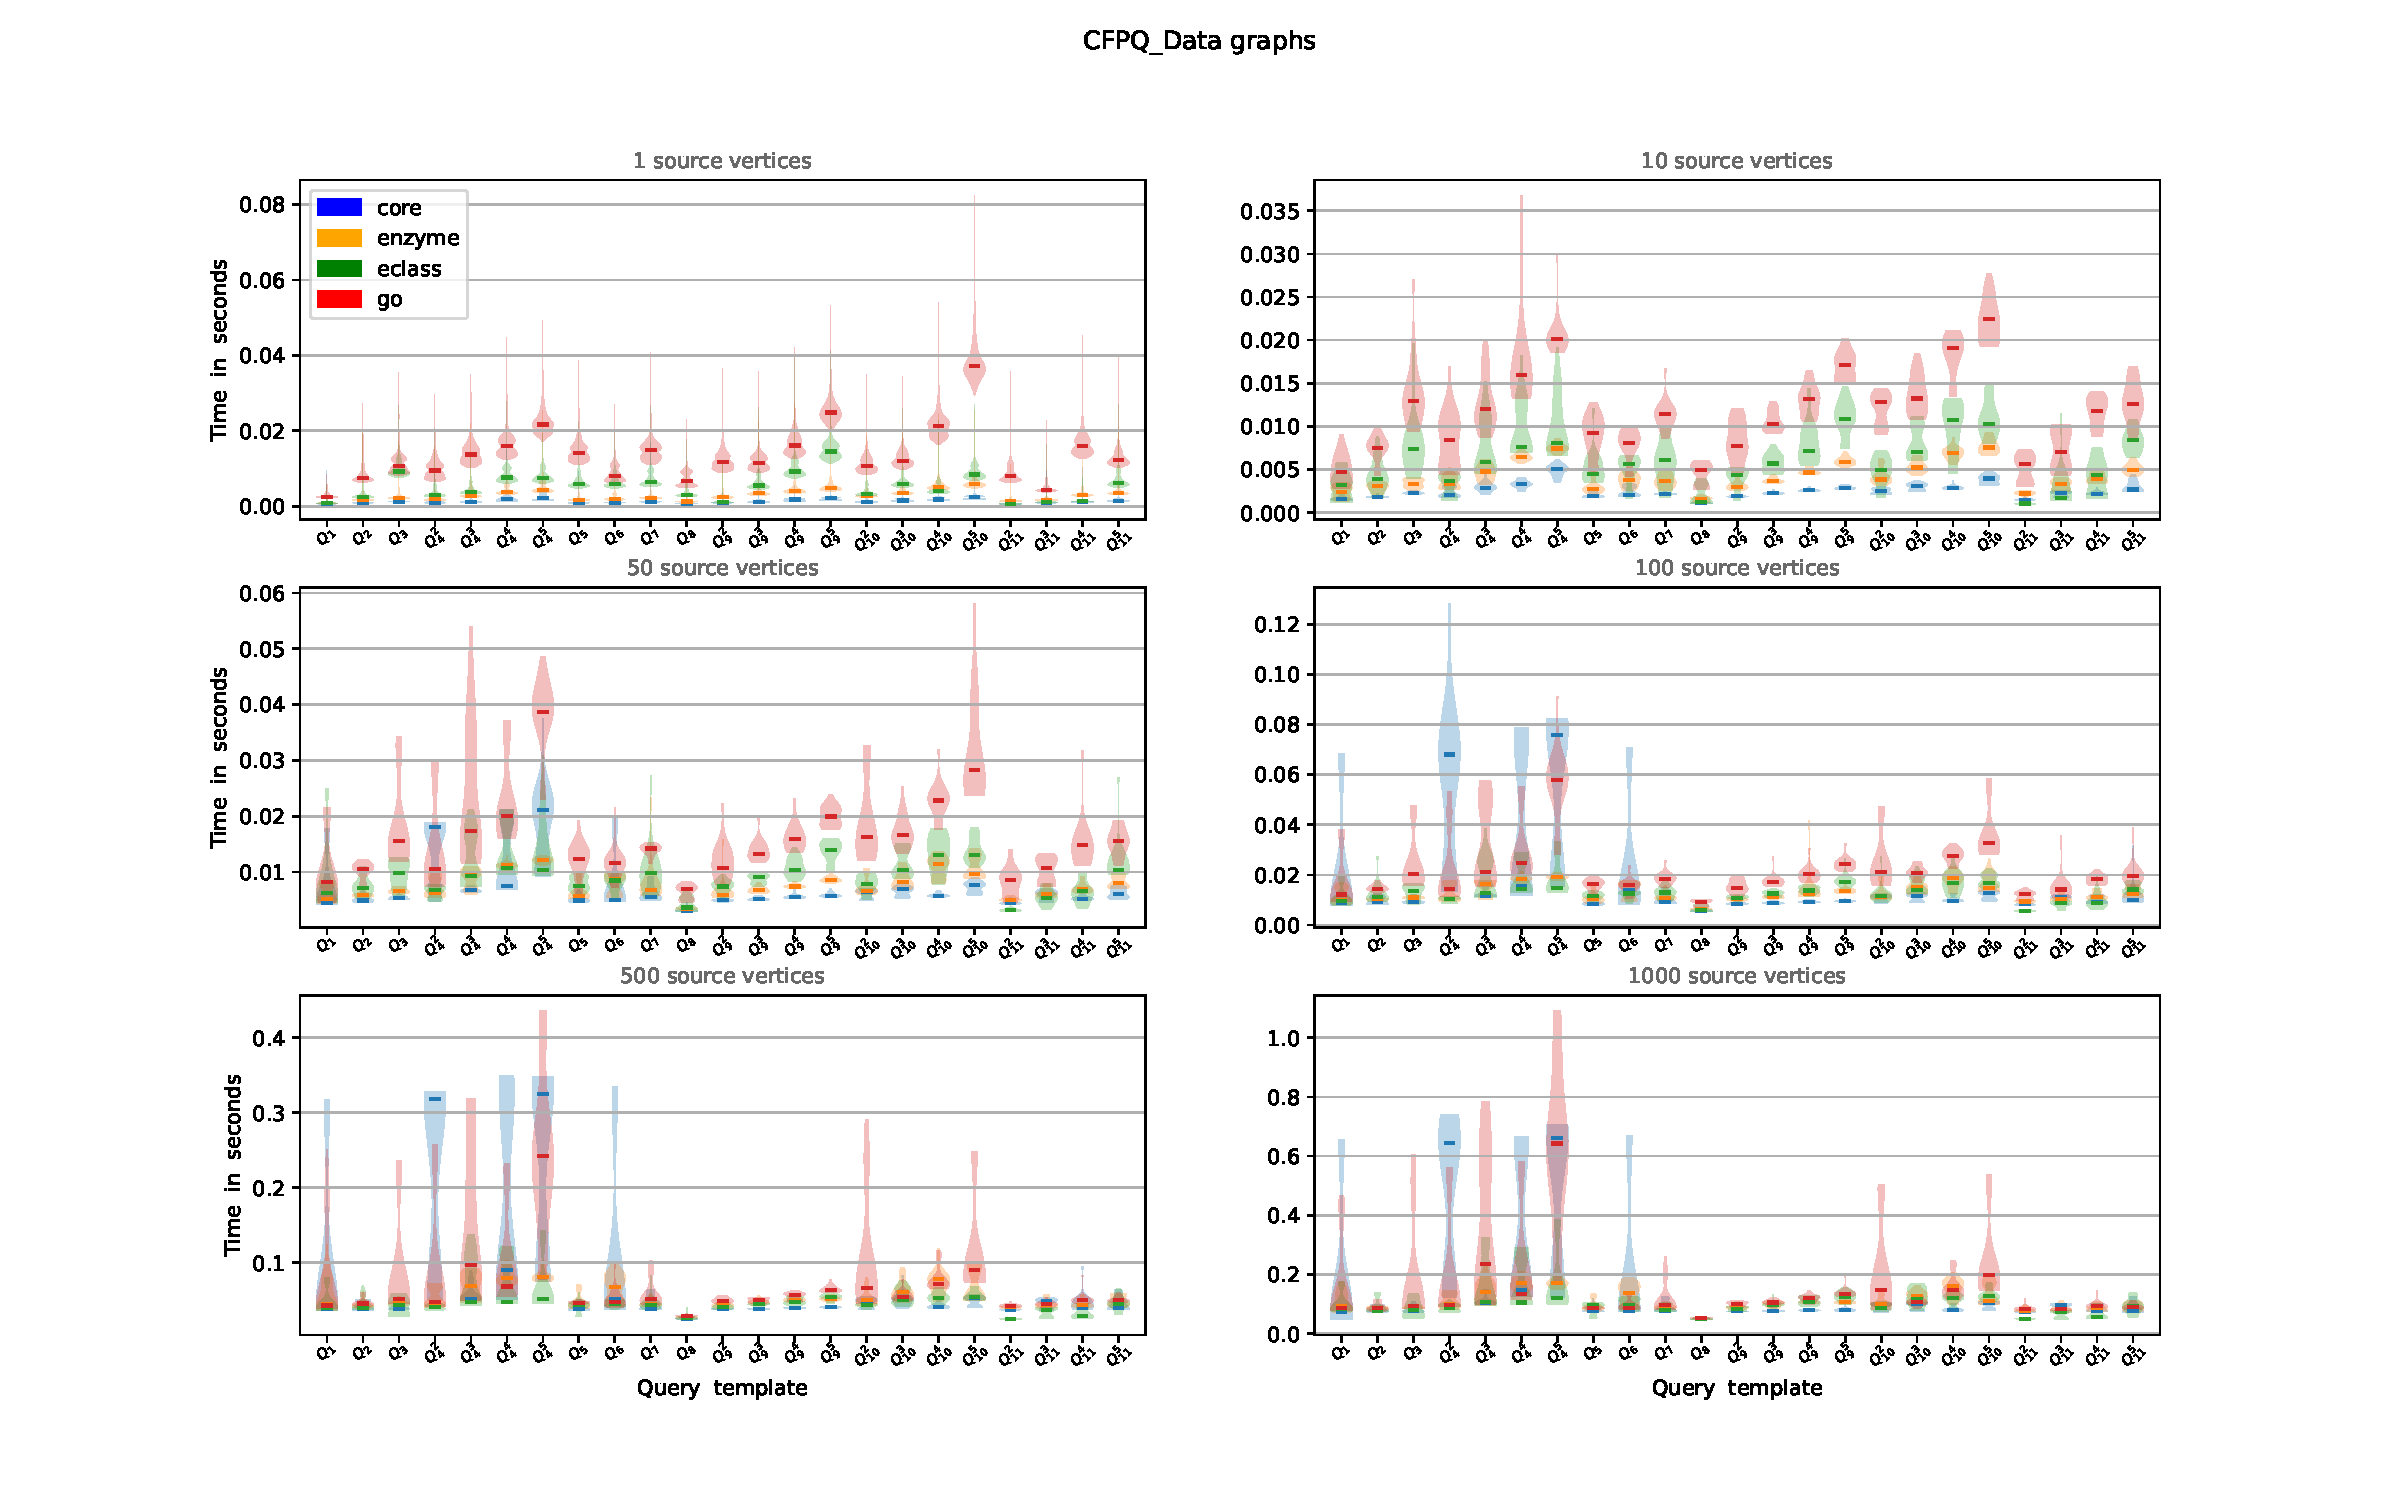
\includegraphics[width=1.4\textwidth]{images/experiment.pdf}}
  \caption{Результаты экспериментов}
  \label{fig:experiment}
\end{figure}

На них продемонстрировано, что разработанный алгоритм достигает скорости работы в доли секунды, что соответствует времени работы аналогичных алгоритмов в научных статьях~\cite{experimet_wang2020}. Это говорит о том, что разработанное решение является конкурентным среди аналогов и может быть эффективно использовано в решении практических задач. Более того, можно сделать следующие выводы:

\begin{itemize}
    \item Производительность алгоритма зависит от сложности запроса. Так, запросы по шаблонам $Q^4_4$, $Q^5_4$ и $Q^4_{10}$, $Q^5_{10}$, содержащие в себе большее количество меток, чем остальные запросы, исполняются в среднем дольше остальных. 
    \item Не всегда время исполнения запроса напрямую зависит от размера графа. Так, при существенном увеличении числа стартовых вершин по отношению к общему числу вершин, алгоритм показывает меньшую производительность. Это заметно на графиках для 100, 500 и 1000 вершин, где вычисления для графа \textit{core} производятся дольше, чем для других графов, имеющих большее число вершин.
    \item Время исполнения запроса редко превышает одну секунду и существенно растет при увеличении числа стартовых вершин.
\end{itemize}
